\chapter{Kube Platform}
In this chapter, we commence on an in-depth exploration of the Kube platform, an implementation of
innovative ERP platform prototype. We start by outlining the fundamental requirements that have
shaped the development of the Kube platform, highlighting the strategic objectives, technical needs,
and business logic that inform its design. This leads us into a detailed examination of the
platform’s final architecture, which showcases a Microservices framework implemented through a
Function as a Service (FaaS) model, using AWS services. We then transition to practical
applications, where specific use cases demonstrate the platform's operational flow and its
real-world applicability. The chapter ends with a focus on the client application, delving into the
design and development of a user interface using Flutter, which not only complements the platform's
robust backend but also enhances the overall user experience. Throughout this chapter, we aim to
unravel the complexities of the Kube platform, illustrating its role as a transformative force in
the field of enterprise resource planning and highlighting its potential.

\section{Requirements}
Before starting development, requirements are established to define the properties of the product.
It's important that these requirements are thorough and coherent, covering all necessary features
without conflicts or inconsistencies. However, creating these documents can be challenging and
errors may occur, such as incomplete or ambiguous feature descriptions, redundancy, or important
details being omitted. To address these challenges, software engineering techniques have been
developed to formalize the requirements and minimize the occurrence of errors.
\newline\newline
ISO/IEC 25010\textsuperscript{\cite{ch5_1}}, an international standard, serves as a comprehensive
framework for assessing software product quality. This standard enumerates several key quality
characteristics, including functionality, reliability, usability, efficiency, maintainability,
security, compatibility, and portability. Its widespread application in software engineering and
quality assurance offers a standardized approach to evaluating and articulating software quality.
This facilitates more informed decisions in software acquisition, development, and maintenance.
ISO/IEC 25010 aids in identifying the actors involved and delineating both functional and
non-functional requirements.

\subsection{Stakeholders}
A stakeholder refers to any role, person, group, or organization that has an interest in a software
project or system being developed. This could include end-users, customers, investors, project
managers, developers and other individuals or groups involved in the development, deployment, and
maintenance of the software. Identifying all relevant stakeholders is important for considering
diverse perspectives and generating relevant requirements for the system. As shown in Table
\ref{tab:5_stakeholders}, numerous stakeholders play a role in the process.

\begin{table}[h]
    \centering
    \begin{tabular}{|l|p{10cm}|}
        \hline
        \textbf{Stakeholder} & \textbf{Description}                                                                                                                                                 \\ \hline
        End-users            & These are the people who will use the ERP system in their day-to-day work. They may include employees from various departments within the organization.              \\ \hline
        Developers           & These are the individuals responsible for creating the software code that makes up the ERP system.                                                                   \\ \hline
        Admin/IT staff       & These are the individuals responsible for installing, configuring, and maintaining the ERP system.                                                                   \\ \hline
        Customers            & These are the organizations or businesses that are purchasing the ERP system. They have a vested interest in ensuring the system meets their needs and requirements. \\ \hline
        Vendors              & These are the organizations that provide the ERP software and related services, such as installation, configuration, and support.                                    \\ \hline
        Cloud Vendors        & These hosts the system and provide the necessary infrastructure for its operation. They are responsible for system availability, scalability, and security.          \\ \hline
    \end{tabular}
    \caption{Stakeholders of a Cloud ERP System.}
    \label{tab:5_stakeholders}
\end{table}

\subsection{Functional and Non-functional}
Functional requirements and non-functional requirements are two types of requirements that are used
to specify what a system or software application should do and how it should perform. They are
important for the successful development and implementation of a system or software application. The
functional requirements ensure that the software application meets the needs of its users, while the
non-functional requirements ensure that the system is reliable, efficient, and secure.

\subsubsection{Functional requirements}
Functional requirements describe what the system should do in terms of its functionalities,
features, and capabilities. They define the specific tasks that the software application should be
able to perform to meet the needs of its users. For distinguish one requirement from another it is
important to assign for each functionality an ID, in order to easy identify it and trace throughout
the life cycle of the project (Table \ref{tab:functional_requirements}).

\begin{table}
    \centering
    \begin{tabular}{|l|p{10cm}|}
        \hline
        ID     & Description                                           \\ \hline
        FR1    & Sign-up users by email and password                   \\ \hline
        FR2    & Login users by email and password                     \\ \hline
        FR3    & Logout users                                          \\ \hline
        FR4    & Activate notifications                                \\ \hline
        FR5    & Deactivate notifications                              \\ \hline
        FR6    & View chart for andamento mensile degli ordini         \\ \hline
        FR7    & View chart for distribuzione degli ordini per cliente \\ \hline
        FR8    & Customize the menu bar                                \\ \hline
        FR9    & View the log of the platform events                   \\ \hline
        FR9.1  & View the detailed log of an event                     \\ \hline
        FR9.2  & Delete a log event                                    \\ \hline
        FR10   & View the customers list                               \\ \hline
        FR10.1 & View the detailed customer                            \\ \hline
        FR10.2 & Insert a customer                                     \\ \hline
        FR10.3 & Update a customer                                     \\ \hline
        FR10.4 & Delete a customer                                     \\ \hline
        FR11   & View the sales order list                             \\ \hline
        FR11.1 & View the detailed sales order with sales lines        \\ \hline
        FR11.2 & Insert a sales order                                  \\ \hline
        FR11.3 & Update a sales order                                  \\ \hline
        FR11.4 & Delete a sales order                                  \\ \hline
        FR11.5 & Insert a sales order line                             \\ \hline
        FR11.6 & Update a sales order line                             \\ \hline
        FR11.7 & Delete a sales order line                             \\ \hline
        FR12   & Launch the posting order event                        \\ \hline
        FR13   & show notifications of change status on order          \\ \hline
        FR14   & View the shipment list                                \\ \hline
        FR14.1 & View the detailed shipment with sales lines           \\ \hline
        FR14.2 & Delete a shipment                                     \\ \hline
        FR15   & View the invoice list                                 \\ \hline
        FR15.1 & View the detailed invoice with sales lines            \\ \hline
        FR15.2 & Delete an invoice                                     \\ \hline
    \end{tabular}
    \caption{Functional requirements for the platform.}
    \label{tab:functional_requirements}
\end{table}

\subsubsection{Non-functional requirements}
Non-functional requirements describe how the system should perform in terms of its functionality,
reliability, usability, efficiency, maintainability, security, compatibility, and portability, all
aspects that are not directly related to the specific functionalities to be implemented. They refer
to operating methods and constraints, such as response times, supported platforms, choice of
languages, required resources, tools and various implementation techniques. They must be measurable
and may be more critical than functional requirements. They are identified with a unique code and it
is also necessary to specify their type associated to the ISO properties and which functional
requirements they refer to (Table \ref{tab:non_functional_requirements}).

\begin{table}
    \centering
    \begin{tabular}{|l|c|p{9cm}|}
        \hline
        ID   & Type            & Description                                                        \\ \hline
        NFR1 & Usabilty        & Application should be used with no training by any user            \\ \hline
        NFR2 & Efficiency      & All functions should complete in < 0.5 sec                         \\ \hline
        NFR2 & Efficiency      & All functions must optimize the resource utilization               \\ \hline
        NFR3 & Portability     & System must work on Chrome, Firefox, Safari, Edge, Android and iOS \\ \hline
        NFR4 & Portability     & No installation is needed                                          \\ \hline
        NFR5 & Compatibility   & Platform must be compatible with Azure and AWS cloud               \\ \hline
        NFR6 & Security        & All data must be stored in a secure database                       \\ \hline
        NFR7 & Maintainability & All functionalities must be tested indipendently                   \\ \hline
        NFR8 & Reliabilty      & Downtime allowed is of one hour per year                           \\ \hline
    \end{tabular}
    \caption{Non-functional requirements for the platform.}
    \label{tab:non_functional_requirements}
\end{table}

\section{Server application}
In this section, we will discuss the final architecture designed for the Kube platform, encompassing
its data structures and services. We will explore the database setup, highlighting the tables
crafted for each microservice. Following this, we'll shed light on the REST APIs tailored for every
microservice, along with the integration of queues and events designed for asynchronous event
management. Concluding our discussion, we'll outline a SAGA implementation that has been
incorporated into the platform.
\newpage

\subsection{Final Architecture}
% TODO Aumenta i font e metti le frecce su events
\begin{figure}
    \centering
    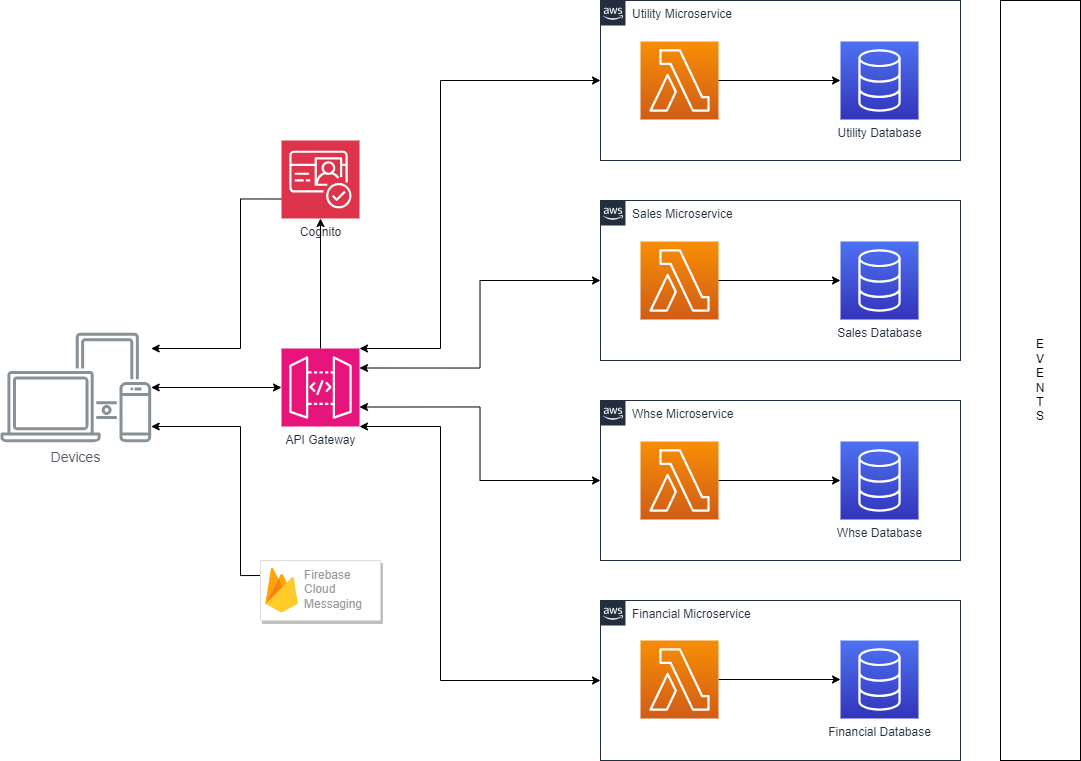
\includegraphics[scale=0.35]{Pictures/5_architecture.png}
    \caption{Final architecture of the platform.}
    \label{fig:5_architecture}
\end{figure}
The architecture diagram in Figure \ref{fig:5_architecture} showcases a modern, serverless
microservices-based architecture for the Kube system. Here's a description based on the elements and
their interconnections:

\begin{itemize}
    \item \textbf{User Authentication}: the service which is responsible for user authentication is
          'Cognito'. It is the entry point for security, ensuring that only authenticated users can
          interact with the platform and with all the API.

    \item \textbf{Firebase Cloud Messaging}: At the bottom of the diagram, we can see 'Firebase Cloud Messaging',
          it is an integration with a cloud solution for sending notifications to devices, allowing for
          real-time user engagement.

    \item \textbf{API Gateway}: The 'API Gateway' is the central hub through which all client
          requests pass. It acts as a front door, directing incoming requests from various devices (such as
          computers and mobile phones) to the appropriate microservices.

    \item \textbf{Microservices Architecture}: Actually each microservice is deployed to AWS (Amazon
          Web Services), and utilize various AWS serverless features for optimizing performance.

          \begin{itemize}
              \item \textbf{Utility Microservice}: This service handles log functions and events,
                    and is backed by a 'Utility Database' for storing log records. It also manage
                    home page graph function and data and navigations/menu API and data.
              \item \textbf{Sales Microservice}: Dedicated to handling sales-related operations,
                    like handle customer and sales order, this service interacts with a 'Sales
                    Database'.
              \item \textbf{Whse Microservice}: this service manages shipment and warehouse-related
                    data, backed by its own 'Whse Database'.
              \item \textbf{Financial Microservice}: This handles financial transactions and invoice, with a
                    separate 'Financial Database' for storing related records.
          \end{itemize}

    \item \textbf{Database Pattern}: The architecture uses a database-per-microservice pattern with SQL
          databases, ensuring that each service has its own datastore, thus maintaining database isolation and
          decoupling services.

    \item \textbf{Event-Driven Architecture}: all microservices are connected through an
          event-driven architecture, which allows them to communicate asynchronously and facilitates
          loose coupling. This architecture is implemented using Amazon Simple Queue Service (SQS)
          and Amazon Simple Notification Service (SNS), which are managed message queues and
          notification services.
\end{itemize}

All services are managed and deployed using the serverless framework, which allows to easily
integrate a CI/CD pipeline manage the entire infrastructure as code. With this setup, the platform
can be easily deployed to other cloud providers and add other cloud services and features. How we
can see, the Kube platform's architecture is designed to be scalable, flexible, and maintainable,
with a focus on modern cloud-native principles and best practices for microservices development.

\subsubsection{Microservices components}
\begin{figure}
    \centering
    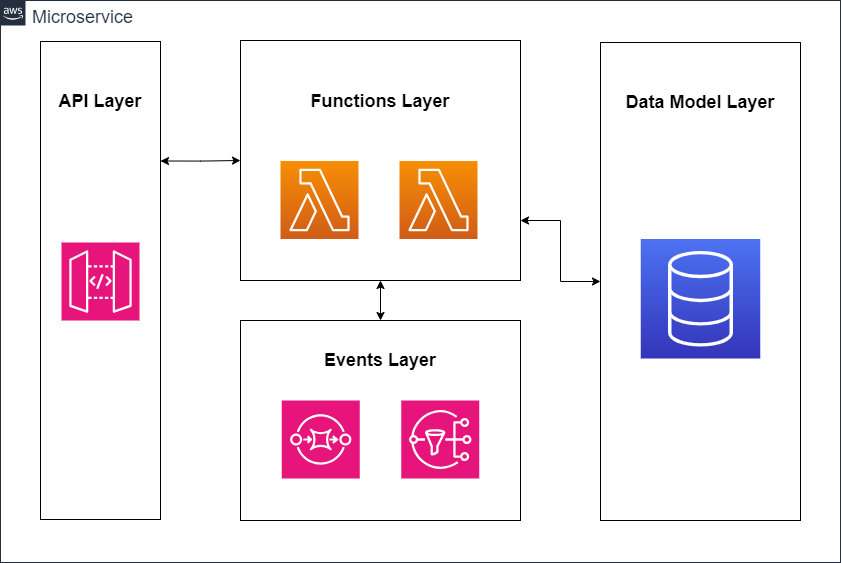
\includegraphics[scale=0.3]{Pictures/5_microservizio.png}
    \caption{Microservices components.}
    \label{fig:5_microservices}
\end{figure}

Each microservice in the Kube platform is a composite of four essential components that work in
concert to deliver its specific functionality:

\begin{table}
    \centering
    \begin{tabular}{|c|c|m{8.5cm}|}
        \hline
        \textbf{Component}   & \textbf{Service} & \textbf{Description}                                                                                                                                                                                                                                                                                                                                                                                                \\ \hline
        \textbf{Data Models} & RDS              & At the core of each microservice is a set of data models. These models define the structure of the data that the microservice handles, ensuring data integrity and consistency. By having its own models, each microservice encapsulates the necessary information to perform its tasks, leading to a clear delineation of responsibilities within the system.                                                      \\ \hline
        \textbf{REST APIs}   & API Gateway      & The REST APIs serve as the interfaces through which external services or client applications interact with the microservices. These APIs are carefully designed to provide a clear and consistent contract for accessing and manipulating data. They follow REST principles, allowing for stateless communication and enabling clients to perform standard HTTP operations such as GET, POST, PATCH, and DELETE.    \\ \hline
        \textbf{Functions}   & Lambda           & The functions are the operational units within each microservice, containing the business logic that processes requests, manipulates data models, and performs the necessary computations. These functions are likely implemented as serverless functions, which are executed in response to events, scaling automatically with the number of requests and reducing the need for managing server infrastructure.    \\ \hline
        \textbf{Events}      & SNS, SQS         & Each microservice also incorporates an event-driven mechanism, signaling and reacting to various conditions and triggers. These events facilitate asynchronous communication between microservices, thereby enhancing the platform's responsiveness and efficiency. By decoupling microservices through events, the system can better handle load variations and failure modes, contributing to overall resilience. \\ \hline
    \end{tabular}
    \caption{Microservices components.}
    \label{tab:microservices_components}
\end{table}

Together, these components create a modular and cohesive microservice that is self-contained,
scalable, and robust. The data models ensure that each service can independently manage its segment
of the data. The REST APIs provide the necessary endpoints for interaction, while the functions
encapsulate the business logic. Finally, the event system allows the services to react to and
communicate changes across the platform without direct coupling, promoting a reactive architecture
that can quickly adapt to changing conditions.
% eventually consistent is enough because not critical data and not all system is coupled

\subsection{Code Structure}
In our microservices architecture, all lambda functions are written in the Go language. This
decision was influenced by several key factors. Firstly, Go is a compiled language, which leads to
significantly faster execution times and results in smaller executable files. Another important
reason for choosing Go is the availability of the Go CDK library. This library is unique to Go and
aids in making functions as portable as possible across different cloud providers. While it's true
that shifting functions between providers requires some manual adjustments, the process could be
streamlined by developing CLI tools for automation.
\newline\newline
However, adopting Go was not without its challenges. Unlike object-oriented languages, Go doesn't
fully integrate all object-oriented principles. It has its own way of handling certain programming
concepts, which required a learning curve. Additionally, Go is not as versatile in some aspects; for
instance, the main function is bound to have a dedicated 'main' package. This can pose difficulties
in managing multiple functions, each with its own 'main,' making the overall management a complex
task.

\begin{figure}
    \centering
    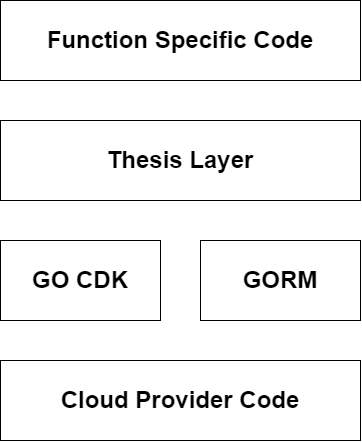
\includegraphics[scale=0.3]{Pictures/5_stack_framework.png}
    \caption{Stack abstractions layer.}
    \label{fig:5_stack_framework}
\end{figure}

In every function architecture, I've implemented an abstraction layer specifically designed for
managing REST APIs of various resources. This unified approach, applied across all microservices, is
facilitated by a layer we've named 'thesis.' Built on top of the GORM and Go CDK libraries, this
layer simplifies and accelerates API management. Connecting a GORM model to a 'thesis' layer
structure called 'page' requires minimal coding. The 'page' concept is central to our approach: it
automatically generates a suite of REST APIs for a resource, significantly reducing development time
and standardizing structures across resources. Moreover, these 'pages' can define a UI schema, which
clients can use to dynamically build pages for resources in their applications. The APIs that are
automatically constructed from a GORM model are structured as indicated inside the following tables.

\subsubsection{http://api.example.com/:pageid?field=value}
\begin{table}
    \centering
    \begin{tabular}{|m{2cm}|m{10cm}|}
        \hline
        \textbf{Method} & \textbf{Description}                                                                                                        \\ \hline
        \textbf{GET}    &
        Returns the list of records linked to the page. The records can be filtered by inserting the fields to be filtered in the URL's query string. \\ \hline
        \textbf{POST}   &
        Creates a new record in the table linked to the page.                                                                                         \\ \hline
        \textbf{PATCH}  &
        Edits the record in the table linked to the page.                                                                                             \\ \hline
        \textbf{DELETE} &
        Deletes records linked to the page. The records can be filtered by inserting the fields to be filtered in the URL's query string.             \\ \hline
    \end{tabular}
    \caption{REST API for page.}
    \label{tab:api_rest_1}
\end{table}

\subsubsection{http://api.example.com/:pageid/schema}
\begin{table}
    \centering
    \begin{tabular}{|m{2cm}|m{10cm}|}
        \hline
        \textbf{Method} & \textbf{Description}                     \\ \hline
        \textbf{GET}    &
        Returns the UI schema for building the page in the client. \\ \hline
        \textbf{POST}   &
        Not allowed.                                               \\ \hline
        \textbf{PATCH}  &
        Not allowed.                                               \\ \hline
        \textbf{DELETE} &
        Not allowed.                                               \\ \hline
    \end{tabular}
    \caption{Methods for page schema.}
    \label{tab:api_rest_2}
\end{table}

\subsubsection{http://api.example.com/:pageid/button?button\_id=value}
\begin{table}
    \centering
    \begin{tabular}{|m{2cm}|m{10cm}|}
        \hline
        \textbf{Method} & \textbf{Description}                                   \\ \hline
        \textbf{GET}    &
        Initiates the functionality linked to the button and returns the result. \\ \hline
        \textbf{POST}   &
        Not allowed.                                                             \\ \hline
        \textbf{PATCH}  &
        Not allowed.                                                             \\ \hline
        \textbf{DELETE} &
        Not allowed.                                                             \\ \hline
    \end{tabular}
    \caption{Methods for page buttons.}
    \label{tab:api_rest_3}
\end{table}

\subsection{Utility Microservice}
% ora entreremo nel dettaglio di ogni microservizio
% spiega come hai strutturato il database per microservizio
% spiega il sistema di notification management
% spiega il sistema di logging
% esso serve a...
\subsubsection{Database}
\subsubsection{API REST}
\subsubsection{Events}
% API REST Create, code SQS create, SNS create, tabelle create
\subsection{Sales Microservice}
\subsection{Whse Microservice}
\subsection{Financial Microservice}

\subsection{Posting Order Event}
% SAGA orchestrated - gaurda il blocco appunti

\section{Client Application}
Client Application: The client application is hosted on GitHub Pages and is integrated with a CI/CD
pipeline using GitHub Actions. This setup automates the deployment process, where any commits pushed
to the repository trigger a build and deployment sequence, ensuring that the latest version of the
web application is always available.

\subsection{Navigation}
\subsection{State Management}
\subsection{Page Builder}

% routing/navigation
% Notification FCM
% authentication
% state management
% page management
% \subsection{User Interface}

\section{Use Case}
A use case comprises various scenarios connected by a shared user objective, serving to illustrate
how a system behaves under different circumstances when processing a request. Each use case should
specify the system as an opaque entity, the user type (often referred to as the actor) interacting
with the system, and the actor's functional objective achieved through the system. A single scenario
represents a series of steps outlining the interaction between a user and the system. Additionally,
each scenario requires a pre-condition that must be met before initiation and a post-condition
fulfilled upon completion. This section will present several use cases, demonstrating the range of
operations a user can execute on the platform.

\subsection{CRUD operations}
\subsection{Posting order}

